\chapter{Combinational Arithmetic Circuits}\label{ch08}
\section{Introduction}

Electronic circuits that do not require any memory devices (like flip-flops or registers) use what is called ``Combinational Logic.'' These systems can be quite complex, but all outputs are determined solely by the actions of a series of logic gates on a given set of inputs. Another characteristic of combinational circuits is the lack of feedback. An output state is determined almost instantly from the inputs with no feedback loops. Combinational circuits can be reduced to a Boolean Algebra expression, though one that may be quite complex. Combinational circuits include many useful applications, including adders, subtractors, multipliers, dividers, encoders, decoders, display drivers, and keyboard encoders.
 
This chapter develops combinational logic circuits.\footnote{All circuits found in this chapter are available as \Le files in the course materials.}

\section{Adders and Subtractors}
\label{CL:sec:adders_and_subtractors}

\subsection{Introduction}
\label{CL:subsec:introduction_to_adders_and_subtractors}

In the Binary Mathematics chapter, the concept of adding two binary numbers was developed and the process of adding binary numbers can be easily implemented in hardware. If two one-bit numbers are added, they will produce a sum and an optional carry-out bit and the circuit that performs this is called a ``half adder.'' If two one-bit numbers along with a carry-in bit from another stage are added they will produce a sum and an optional carry-out, and the circuit that performs this is function called a ``full adder.'' 

Subtractors are similar to adders but they must be able to signal a ``borrow'' bit rather than send a carry-out bit. Like adders, subtractors are developed from half-subtractor circuits. This unit develops both adders and subtractors.

\subsection{Half Adder}
\label{CL:subsec:half_adder}

Following is the truth table for a half adder.

\begin{table}[H]
  \sffamily
  \newcommand{\head}[1]{\textcolor{white}{\textbf{#1}}}    
  \begin{center}
    \rowcolors{2}{gray!10}{white} % Color every other line a light gray
    \begin{tabular}{cc|cc} 
      \rowcolor{black!75}
      \multicolumn{2}{c}{\head{Inputs}} & \multicolumn{2}{c}{\head{Output}} \\
      A & B & Sum & COut \\
      \hline
      0 & 0 & 0 & 0 \\
      0 & 1 & 1 & 0 \\
      1 & 0 & 1 & 0 \\
      1 & 1 & 0 & 1 
    \end{tabular}
  \end{center}
  \caption{Truth Table for Half-Adder}
  \label{CL:tab:truth_table_for_half_adder}
\end{table}

The \emph{Sum} column in this truth table is the same pattern as an \textsf{XOR}) so the easiest way to create a half adder is to use an \textsf{XOR} gate. However, if both input bits are high a half adder will also generate a carry out (\emph{COut}) bit, so the half adder circuit should be designed to provide that carry out. The circuit in Figure \ref{fig:08_05} meets those requirements. In this circuit, \emph{A} and \emph{B} are connected to \textsf{XOR} gate \textsf{U1} and that is connected to output \emph{Sum}. \emph{A} and \emph{B} are also connected to \textsf{AND} gate \textsf{U2} and that is connected to carry-out bit \emph{COut}.

\begin{figure}[H]
	\centering
	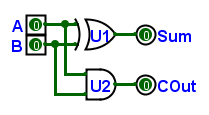
\includegraphics[width=\maxwidth{.95\linewidth}]{gfx/08_05}
	\caption{Half-Adder}
	\label{fig:08_05}
\end{figure}

\subsection{Full Adder}
\label{CL:subsec:full_adder}

A full adder sums two one-bit numbers along with a carry-in bit and produces a sum with a carry-out bit. Truth table \ref{CL:tab:truth_table_for_full_adder} defines a full adder. 

\begin{table}[H]
  \sffamily
  \newcommand{\head}[1]{\textcolor{white}{\textbf{#1}}}    
  \begin{center}
    \rowcolors{2}{gray!10}{white} % Color every other line a light gray
    \begin{tabular}{ccc|cc} 
      \rowcolor{black!75}
      \multicolumn{3}{c}{\head{Inputs}} & \multicolumn{2}{c}{\head{Output}} \\
      A & B & CIn & Sum & COut \\
      \hline
      0 & 0 & 0 & 0 & 0 \\
      0 & 0 & 1 & 1 & 0 \\
      0 & 1 & 0 & 1 & 0 \\
      0 & 1 & 1 & 0 & 1 \\
      1 & 0 & 0 & 1 & 0 \\
      1 & 0 & 1 & 0 & 1 \\
      1 & 1 & 0 & 0 & 1 \\
      1 & 1 & 1 & 1 & 1
    \end{tabular}
  \end{center}
  \caption{Truth Table for Full Adder}
  \label{CL:tab:truth_table_for_full_adder}
\end{table}

Following are Karnaugh Maps for both outputs.

%%%%%%%%%%%%%%%%%%%%%%%%%%%%%%%%%%%%%%%%%%%%%%%
%%% K-Map for Sum
%%%%%%%%%%%%%%%%%%%%%%%%%%%%%%%%%%%%%%%%%%%%%%%
\begin{figure}[H]
	\myfloatalign
	\begin{tikzpicture} [circuit logic US, scale=1.00]
	% make all path lines (the node shapes) a little thicker
	\tikzstyle{every path}=[line width=0.50mm]
	
	%********************************************************************
	% Adjust the settings below to display the 1's and rectangles
	%********************************************************************
	% Uncomment the appropriate lines below to insert ones where needed
	%   \node[] at (2.25,2.25) {\Huge $ 1 $}; % 00
	   \node[] at (2.25,0.75) {\Huge $ 1 $}; % 01
	   \node[] at (3.75,2.25) {\Huge $ 1 $}; % 02
	%   \node[] at (3.75,0.75) {\Huge $ 1 $}; % 03
	   \node[] at (6.75,2.25) {\Huge $ 1 $}; % 04
	%   \node[] at (6.75,0.75) {\Huge $ 1 $}; % 05
	%   \node[] at (5.25,2.25) {\Huge $ 1 $}; % 06
	   \node[] at (5.25,0.75) {\Huge $ 1 $}; % 07
	
	% The coords for each cell - this is used as the origin for the solution box
	\coordinate (cell00) at (1.5,1.5); \coordinate (cell01) at (1.5,0.0);
	\coordinate (cell02) at (3.0,1.5); \coordinate (cell03) at (3.0,0.0);
	
	\coordinate (cell04) at (6.0,1.5); \coordinate (cell05) at (6.0,0.0);
	\coordinate (cell06) at (4.5,1.5); \coordinate (cell07) at (4.5,0.0);
	
	% The colored boxes enclosing adjacent ones
	% Set the ``at'' to the lower-left cell of the rectangle using 
	% the 'cellxx' defined above
	% Set the minimum height/width to (number of cells) * 1.5. 
	% May have to decrease these by 0.1 to cut the rectangle 
	% just inside the cell.
	\node [draw,
	color=yellow!70!black,
	fill=yellow!20!white,
	fill opacity=0.3,
	minimum height=1.4cm,
	minimum width=1.4cm,
	double,
	rounded corners,
	anchor=south west] at (cell01) {};
	
	\node [draw,
	color=yellow!70!black,
	fill=yellow!20!white,
	fill opacity=0.3,
	minimum height=1.4cm,
	minimum width=1.4cm,
	double,
	rounded corners,
	anchor=south west] at (cell02) {};

	\node [draw,
	color=yellow!70!black,
	fill=yellow!20!white,
	fill opacity=0.3,
	minimum height=1.4cm,
	minimum width=1.4cm,
	double,
	rounded corners,
	anchor=south west] at (cell07) {};

	\node [draw,
	color=yellow!70!black,
	fill=yellow!20!white,
	fill opacity=0.3,
	minimum height=1.4cm,
	minimum width=1.4cm,
	double,
	rounded corners,
	anchor=south west] at (cell04) {};

	%********************************************************************
	% Shouldn't need to adjust anything below this point - this is just
	% the grid and the minterms.
	%********************************************************************  
	% Text in top-Left cell
	\node[] at (0.50,3.40) { $ \mathsf{ \mathbf{C} } $ }; % C
	\node[] at (1.10,4.05) { $ \mathsf{ \mathbf{AB} } $ }; % AB
	
	% Populate the top row header
	% In the following, the foreach lists a location/text pair
	% The the draw line draws the text at each location
	\foreach \loc/\txt in {
		(2.25,3.75)/{00}, (3.75,3.75)/{01},
		(5.25,3.75)/{11}, (6.75,3.75)/{10}
	}
	\draw \loc node{\Huge $\txt$};
	
	% Populate the header in column one
	\foreach \loc/\txt in { 
		(0.75,2.25)/{0},(0.75,0.75)/{1}
	}
	\draw \loc node{\Huge $\txt$};
	
	% Populate the minterms
	\foreach \loc/\txt in { 
		(2.75,1.75)/{00} , (4.25,1.75)/{02} , (5.75,1.75)/{06} , (7.25,1.75)/{04} ,
		(2.75,0.15)/{01} , (4.25,0.15)/{03} , (5.75,0.15)/{07} , (7.25,0.15)/{05} }
	\draw \loc node{ \color{blue!90!black} \small { $\txt$ }};
	
	% Draw the lines
	\draw
	% Finish drawing the grid
	[step=1.5cm,black,thin] (0,0) grid (7.5,4.5) % The Grid
	(0.0,4.5) -- (1.5,3.0) % Diagonal in the top left cell
	(1.5,3.10) -- (7.5,3.10) % Double line under top header row
	(1.40,0.0) -- (1.40,3.0) % Double line on left of header column one
	;    
	\end{tikzpicture}
	\caption{K-Map For The SUM Output}
	\label{kmap:08_01}
\end{figure}



%%%%%%%%%%%%%%%%%%%%%%%%%%%%%%%%%%%%%%%%%%%%%%%
%%% K-Map for COut
%%%%%%%%%%%%%%%%%%%%%%%%%%%%%%%%%%%%%%%%%%%%%%%
\begin{figure}[H]
	\myfloatalign
	\begin{tikzpicture} [circuit logic US, scale=1.00]
	% make all path lines (the node shapes) a little thicker
	\tikzstyle{every path}=[line width=0.50mm]
	
	%********************************************************************
	% Adjust the settings below to display the 1's and rectangles
	%********************************************************************
	% Uncomment the appropriate lines below to insert ones where needed
	%   \node[] at (2.25,2.25) {\Huge $ 1 $}; % 00
	%   \node[] at (2.25,0.75) {\Huge $ 1 $}; % 01
	%   \node[] at (3.75,2.25) {\Huge $ 1 $}; % 02
	   \node[] at (3.75,0.75) {\Huge $ 1 $}; % 03
	%   \node[] at (6.75,2.25) {\Huge $ 1 $}; % 04
	   \node[] at (6.75,0.75) {\Huge $ 1 $}; % 05
	   \node[] at (5.25,2.25) {\Huge $ 1 $}; % 06
	   \node[] at (5.25,0.75) {\Huge $ 1 $}; % 07
	
	% The coords for each cell - this is used as the origin for the solution box
	\coordinate (cell00) at (1.5,1.5); \coordinate (cell01) at (1.5,0.0);
	\coordinate (cell02) at (3.0,1.5); \coordinate (cell03) at (3.0,0.0);
	
	\coordinate (cell04) at (6.0,1.5); \coordinate (cell05) at (6.0,0.0);
	\coordinate (cell06) at (4.5,1.5); \coordinate (cell07) at (4.5,0.0);
	
	% The colored boxes enclosing adjacent ones
	% Set the ``at'' to the lower-left cell of the rectangle using 
	% the 'cellxx' defined above
	% Set the minimum height/width to (number of cells) * 1.5. 
	% May have to decrease these by 0.1 to cut the rectangle 
	% just inside the cell.
	\node [draw,
	color=red!70!black,
	fill=red!20!white,
	fill opacity=0.3,
	minimum height=1.4cm,
	minimum width=2.9cm,
	double,
	rounded corners,
	anchor=south west] at (cell03) {};

	\node [draw,
	color=green!70!black,
	fill=green!20!white,
	fill opacity=0.3,
	minimum height=1.4cm,
	minimum width=2.9cm,
	double,
	rounded corners,
	anchor=south west] at (cell07) {};
	
	\node [draw,
	color=blue!70!black,
	fill=blue!20!white,
	fill opacity=0.3,
	minimum height=2.9cm,
	minimum width=1.5cm,
	double,
	rounded corners,
	anchor=south west] at (cell07) {};
	
	%********************************************************************
	% Shouldn't need to adjust anything below this point - this is just
	% the grid and the minterms.
	%********************************************************************  
	% Text in top-Left cell
	\node[] at (0.50,3.40) { $ \mathsf{ \mathbf{C} } $ }; % C
	\node[] at (1.10,4.05) { $ \mathsf{ \mathbf{AB} } $ }; % AB
	
	% Populate the top row header
	% In the following, the foreach lists a location/text pair
	% The the draw line draws the text at each location
	\foreach \loc/\txt in {
		(2.25,3.75)/{00}, (3.75,3.75)/{01},
		(5.25,3.75)/{11}, (6.75,3.75)/{10}
	}
	\draw \loc node{\Huge $\txt$};
	
	% Populate the header in column one
	\foreach \loc/\txt in { 
		(0.75,2.25)/{0},(0.75,0.75)/{1}
	}
	\draw \loc node{\Huge $\txt$};
	
	% Populate the minterms
	\foreach \loc/\txt in { 
		(2.75,1.75)/{00} , (4.25,1.75)/{02} , (5.75,1.75)/{06} , (7.25,1.75)/{04} ,
		(2.75,0.15)/{01} , (4.25,0.15)/{03} , (5.75,0.15)/{07} , (7.25,0.15)/{05} }
	\draw \loc node{ \color{blue!90!black} \small { $\txt$ }};
	
	% Draw the lines
	\draw
	% Finish drawing the grid
	[step=1.5cm,black,thin] (0,0) grid (7.5,4.5) % The Grid
	(0.0,4.5) -- (1.5,3.0) % Diagonal in the top left cell
	(1.5,3.10) -- (7.5,3.10) % Double line under top header row
	(1.40,0.0) -- (1.40,3.0) % Double line on left of header column one
	;    
	\end{tikzpicture}
	\caption{K-Map For The COut Output}
	\label{kmap:08_02}
\end{figure}

Karnaugh map \ref{kmap:08_01} is a Reed-Muller pattern that is typical of an \textsf{XOR} gate. Karnaugh map \ref{kmap:08_02} can be reduced to three Boolean expressions. The full adder circuit is, therefore, defined by the following Boolean equations. 

\begin{align}
  \label{CL:eq:full_adder}
  A \oplus B \oplus CIn &= Sum \\
  \nonumber
  (A * B) + (A * CIn) + (B * CIn) &= COut
\end{align}

Figure \ref{fig:08_06} is a full adder. In essence, this circuit combines two half-adders such that \textsf{U1} and \textsf{U2} are one half-adder that sums \emph{A} and \emph{B} while \textsf{U3} and \textsf{U4} are the other half-adder that sums the output of the first half-adder and \emph{CIn}.

\begin{figure}[H]
	\centering
	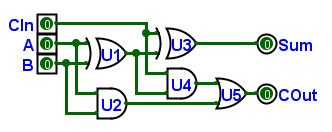
\includegraphics[width=\maxwidth{.95\linewidth}]{gfx/08_06}
	\caption{Full Adder}
	\label{fig:08_06}
\end{figure}

\subsection{Cascading Adders}
\label{CL:subsec:cascading_adders}

The full adder developed above will only add two one-bit numbers along with an optional carry-in bit; however, those adders can be cascaded such that an adder of any bit width can be easily created. Figure \ref{fig:08_07} shows a four-bit adder created by cascading four one-bit adders. 

\begin{figure}[H]
	\centering
	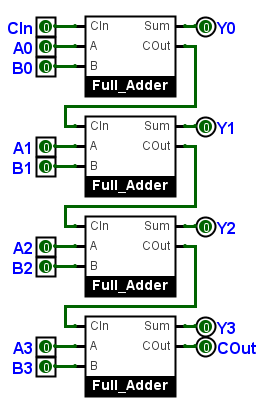
\includegraphics[width=\maxwidth{.95\linewidth}]{gfx/08_07}
	\caption{4-Bit Adder}
	\label{fig:08_07}
\end{figure}

This circuit would add two four-bit inputs, \emph{A} and \emph{B}. Stage zero, at the top of the stack, adds bit zero from both inputs and then outputs bit zero of the sum, \emph{Y0}, along with a carry-out bit. The carry-out bit from stage zero is wired directly into the stage one's carry-in port. That adder then adds bit one from both inputs along with the carry-in bit to create bit one of the sum, \emph{Y1}, along with a carry-out bit. This process continues until all for bits have been added. In the end, outputs \emph{Y0} - \emph{Y3} are combined to create a four-bit sum. If there is a carry-out bit from the last stage it could be used as the carry-in bit for another device or could be used to signal an overflow error.

\subsection{Half Subtractor}
\label{CL:subsec:half_subtractor}

To understand a binary subtraction circuit, it is helpful begin with subtraction in a base-10 system.  

\begin{binDisp}[commandchars=~\[\]]
     83
    -~underline[65]
     18
\end{binDisp}

Since $ 5 $ cannot be subtracted from $ 3 $ (the least significant digits), $ 10 $ must be borrowed from $ 8 $. This is simple elementary-school arithmetic but the principle is important for base-2 subtraction. There are only four possible one-bit subtraction problems.

\begin{binDisp}[commandchars=~\[\]]
     0     1     1     10
    -~underline[0]    -~underline[0]    -~underline[1]     -~underline[1]
     0     1     0      1
\end{binDisp}

The first three examples above need no explanation, but the fourth only makes sense when it is understood that it is impossible to subtract $ 1 $ from $ 0 $ so $ 10_{2} $ was borrowed from the next most significant bit position. The problems above were used to generate the following half-subtractor truth table.

\begin{table}[H]
	\sffamily
	\newcommand{\head}[1]{\textcolor{white}{\textbf{#1}}}    
	\begin{center}
		\rowcolors{2}{gray!10}{white} % Color every other line a light gray
		\begin{tabular}{ccc|cc} 
			\rowcolor{black!75}
			\multicolumn{2}{c}{\head{Inputs}} & \multicolumn{2}{c}{\head{Outputs}} \\
			A & B & Diff & BOut \\
			\hline
			0 & 0 & 0 & 0 \\
			0 & 1 & 1 & 1 \\
			1 & 0 & 1 & 0 \\
			1 & 1 & 0 & 0
		\end{tabular}
	\end{center}
	\caption{Truth Table for Half-Subtractor}
	\label{CL:tab:truth_table_for_half_subtractor}
\end{table}

\emph{Diff} is the difference of \emph{A} minus \emph{B}. \emph{BOut} (``Borrow Out'') is a signal that a borrow is necessary from the next most significant bit position when \emph{B} is greater than \emph{A}. The following Boolean equations define the calculations needed for a half-subtractor.

\begin{align}
\label{CL:eq:half_subtractor}
	A \oplus B &= Diff \\
	\nonumber
	A' * B &= BOut
\end{align}

The pattern for \emph{Diff} is the same as an \textsf{XOR} gate so using an \textsf{XOR} gate is the easiest way to generate the difference. \emph{BOut} is only high when \emph{A} is low and \emph{B} is high so a simple \textsf{AND} gate with one inverted input can be used to generate \emph{BOut}. The circuit in figure \ref{fig:08_08} realizes a half-subtractor.

\begin{figure}[H]
	\centering
	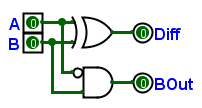
\includegraphics[width=\maxwidth{.95\linewidth}]{gfx/08_08}
	\caption{Half-Subtractor}
	\label{fig:08_08}
\end{figure}

\subsection{Full Subtractor}
\label{CL:subsec:full_subtractor}

A full subtractor produces a difference and borrow-out signal, just like a half-subtractor, but also includes a borrow-in signal so they can be cascaded to create a subtractor of any desired bit width.

Truth table \ref{CL:tab:truth_table_for_subtractor} is for a full subtractor. 

\begin{table}[H]
	\sffamily
	\newcommand{\head}[1]{\textcolor{white}{\textbf{#1}}}    
	\begin{center}
		\rowcolors{2}{gray!10}{white} % Color every other line a light gray
		\begin{tabular}{ccc|cc} 
			\rowcolor{black!75}
			\multicolumn{3}{c}{\head{Inputs}} & \multicolumn{2}{c}{\head{Output}} \\
			A & B & BIn & Diff & BOut \\
			\hline
			0 & 0 & 0 & 0 & 0 \\
			0 & 0 & 1 & 1 & 1 \\
			0 & 1 & 0 & 1 & 1 \\
			0 & 1 & 1 & 0 & 1 \\
			1 & 0 & 0 & 1 & 0 \\
			1 & 0 & 1 & 0 & 0 \\
			1 & 1 & 0 & 0 & 0 \\
			1 & 1 & 1 & 1 & 1
		\end{tabular}
	\end{center}
	\caption{Truth Table for Subtractor}
	\label{CL:tab:truth_table_for_subtractor}
\end{table}

\emph{Diff} is the difference of \emph{A} minus \emph{B} minus \emph{BIn}. \emph{BOut} (``Borrow Out'') is a signal that a borrow is necessary from the next most significant bit position when \emph{A} is less than \emph{B} plus \emph{BIn}. 

Following are Karnaugh Maps for both outputs.

%%%%%%%%%%%%%%%%%%%%%%%%%%%%%%%%%%%%%%%%%%%%%%%
%%% K-Map for Difference
%%%%%%%%%%%%%%%%%%%%%%%%%%%%%%%%%%%%%%%%%%%%%%%
\begin{figure}[H]
	\myfloatalign
	\begin{tikzpicture} [circuit logic US, scale=1.00]
	% make all path lines (the node shapes) a little thicker
	\tikzstyle{every path}=[line width=0.50mm]
	
	%********************************************************************
	% Adjust the settings below to display the 1's and rectangles
	%********************************************************************
	% Uncomment the appropriate lines below to insert ones where needed
	%   \node[] at (2.25,2.25) {\Huge $ 1 $}; % 00
	\node[] at (2.25,0.75) {\Huge $ 1 $}; % 01
	\node[] at (3.75,2.25) {\Huge $ 1 $}; % 02
	%   \node[] at (3.75,0.75) {\Huge $ 1 $}; % 03
	\node[] at (6.75,2.25) {\Huge $ 1 $}; % 04
	%   \node[] at (6.75,0.75) {\Huge $ 1 $}; % 05
	%   \node[] at (5.25,2.25) {\Huge $ 1 $}; % 06
	\node[] at (5.25,0.75) {\Huge $ 1 $}; % 07
	
	% The coords for each cell - this is used as the origin for the solution box
	\coordinate (cell00) at (1.5,1.5); \coordinate (cell01) at (1.5,0.0);
	\coordinate (cell02) at (3.0,1.5); \coordinate (cell03) at (3.0,0.0);
	
	\coordinate (cell04) at (6.0,1.5); \coordinate (cell05) at (6.0,0.0);
	\coordinate (cell06) at (4.5,1.5); \coordinate (cell07) at (4.5,0.0);
	
	% The colored boxes enclosing adjacent ones
	% Set the ``at'' to the lower-left cell of the rectangle using 
	% the 'cellxx' defined above
	% Set the minimum height/width to (number of cells) * 1.5. 
	% May have to decrease these by 0.1 to cut the rectangle 
	% just inside the cell.
	\node [draw,
	color=yellow!70!black,
	fill=yellow!20!white,
	fill opacity=0.3,
	minimum height=1.4cm,
	minimum width=1.4cm,
	double,
	rounded corners,
	anchor=south west] at (cell01) {};
	
	\node [draw,
	color=yellow!70!black,
	fill=yellow!20!white,
	fill opacity=0.3,
	minimum height=1.4cm,
	minimum width=1.4cm,
	double,
	rounded corners,
	anchor=south west] at (cell02) {};
	
	\node [draw,
	color=yellow!70!black,
	fill=yellow!20!white,
	fill opacity=0.3,
	minimum height=1.4cm,
	minimum width=1.4cm,
	double,
	rounded corners,
	anchor=south west] at (cell07) {};
	
	\node [draw,
	color=yellow!70!black,
	fill=yellow!20!white,
	fill opacity=0.3,
	minimum height=1.4cm,
	minimum width=1.4cm,
	double,
	rounded corners,
	anchor=south west] at (cell04) {};
	
	%********************************************************************
	% Shouldn't need to adjust anything below this point - this is just
	% the grid and the minterms.
	%********************************************************************  
	% Text in top-Left cell
	\node[] at (0.50,3.40) { $ \mathsf{ \mathbf{C} } $ }; % C
	\node[] at (1.10,4.05) { $ \mathsf{ \mathbf{AB} } $ }; % AB
	
	% Populate the top row header
	% In the following, the foreach lists a location/text pair
	% The the draw line draws the text at each location
	\foreach \loc/\txt in {
		(2.25,3.75)/{00}, (3.75,3.75)/{01},
		(5.25,3.75)/{11}, (6.75,3.75)/{10}
	}
	\draw \loc node{\Huge $\txt$};
	
	% Populate the header in column one
	\foreach \loc/\txt in { 
		(0.75,2.25)/{0},(0.75,0.75)/{1}
	}
	\draw \loc node{\Huge $\txt$};
	
	% Populate the minterms
	\foreach \loc/\txt in { 
		(2.75,1.75)/{00} , (4.25,1.75)/{02} , (5.75,1.75)/{06} , (7.25,1.75)/{04} ,
		(2.75,0.15)/{01} , (4.25,0.15)/{03} , (5.75,0.15)/{07} , (7.25,0.15)/{05} }
	\draw \loc node{ \color{blue!90!black} \small { $\txt$ }};
	
	% Draw the lines
	\draw
	% Finish drawing the grid
	[step=1.5cm,black,thin] (0,0) grid (7.5,4.5) % The Grid
	(0.0,4.5) -- (1.5,3.0) % Diagonal in the top left cell
	(1.5,3.10) -- (7.5,3.10) % Double line under top header row
	(1.40,0.0) -- (1.40,3.0) % Double line on left of header column one
	;    
	\end{tikzpicture}
	\caption{K-Map For The Difference Output}
	\label{kmap:08_03}
\end{figure}



%%%%%%%%%%%%%%%%%%%%%%%%%%%%%%%%%%%%%%%%%%%%%%%
%%% K-Map for BOut
%%%%%%%%%%%%%%%%%%%%%%%%%%%%%%%%%%%%%%%%%%%%%%%
\begin{figure}[H]
	\myfloatalign
	\begin{tikzpicture} [circuit logic US, scale=1.00]
	% make all path lines (the node shapes) a little thicker
	\tikzstyle{every path}=[line width=0.50mm]
	
	%********************************************************************
	% Adjust the settings below to display the 1's and rectangles
	%********************************************************************
	% Uncomment the appropriate lines below to insert ones where needed
	%   \node[] at (2.25,2.25) {\Huge $ 1 $}; % 00
	   \node[] at (2.25,0.75) {\Huge $ 1 $}; % 01
	   \node[] at (3.75,2.25) {\Huge $ 1 $}; % 02
	   \node[] at (3.75,0.75) {\Huge $ 1 $}; % 03
	%   \node[] at (6.75,2.25) {\Huge $ 1 $}; % 04
	%   \node[] at (6.75,0.75) {\Huge $ 1 $}; % 05
	%   \node[] at (5.25,2.25) {\Huge $ 1 $}; % 06
	   \node[] at (5.25,0.75) {\Huge $ 1 $}; % 07
	
	% The coords for each cell - this is used as the origin for the solution box
	\coordinate (cell00) at (1.5,1.5); \coordinate (cell01) at (1.5,0.0);
	\coordinate (cell02) at (3.0,1.5); \coordinate (cell03) at (3.0,0.0);
	
	\coordinate (cell04) at (6.0,1.5); \coordinate (cell05) at (6.0,0.0);
	\coordinate (cell06) at (4.5,1.5); \coordinate (cell07) at (4.5,0.0);
	
	% The colored boxes enclosing adjacent ones
	% Set the ``at'' to the lower-left cell of the rectangle using 
	% the 'cellxx' defined above
	% Set the minimum height/width to (number of cells) * 1.5. 
	% May have to decrease these by 0.1 to cut the rectangle 
	% just inside the cell.
	\node [draw,
	color=red!70!black,
	fill=red!20!white,
	fill opacity=0.3,
	minimum height=1.4cm,
	minimum width=2.9cm,
	double,
	rounded corners,
	anchor=south west] at (cell01) {};
	
	\node [draw,
	color=green!70!black,
	fill=green!20!white,
	fill opacity=0.3,
	minimum height=1.4cm,
	minimum width=2.9cm,
	double,
	rounded corners,
	anchor=south west] at (cell03) {};
	
	\node [draw,
	color=blue!70!black,
	fill=blue!20!white,
	fill opacity=0.3,
	minimum height=2.9cm,
	minimum width=1.5cm,
	double,
	rounded corners,
	anchor=south west] at (cell03) {};
	
	%********************************************************************
	% Shouldn't need to adjust anything below this point - this is just
	% the grid and the minterms.
	%********************************************************************  
	% Text in top-Left cell
	\node[] at (0.50,3.40) { $ \mathsf{ \mathbf{C} } $ }; % C
	\node[] at (1.10,4.05) { $ \mathsf{ \mathbf{AB} } $ }; % AB
	
	% Populate the top row header
	% In the following, the foreach lists a location/text pair
	% The the draw line draws the text at each location
	\foreach \loc/\txt in {
		(2.25,3.75)/{00}, (3.75,3.75)/{01},
		(5.25,3.75)/{11}, (6.75,3.75)/{10}
	}
	\draw \loc node{\Huge $\txt$};
	
	% Populate the header in column one
	\foreach \loc/\txt in { 
		(0.75,2.25)/{0},(0.75,0.75)/{1}
	}
	\draw \loc node{\Huge $\txt$};
	
	% Populate the minterms
	\foreach \loc/\txt in { 
		(2.75,1.75)/{00} , (4.25,1.75)/{02} , (5.75,1.75)/{06} , (7.25,1.75)/{04} ,
		(2.75,0.15)/{01} , (4.25,0.15)/{03} , (5.75,0.15)/{07} , (7.25,0.15)/{05} }
	\draw \loc node{ \color{blue!90!black} \small { $\txt$ }};
	
	% Draw the lines
	\draw
	% Finish drawing the grid
	[step=1.5cm,black,thin] (0,0) grid (7.5,4.5) % The Grid
	(0.0,4.5) -- (1.5,3.0) % Diagonal in the top left cell
	(1.5,3.10) -- (7.5,3.10) % Double line under top header row
	(1.40,0.0) -- (1.40,3.0) % Double line on left of header column one
	;    
	\end{tikzpicture}
	\caption{K-Map For The BOut Output}
	\label{kmap:08_04}
\end{figure}

Karnaugh map \ref{kmap:08_03} is a Reed-Muller pattern that is typical of an \textsf{XOR} gate. Karnaugh map \ref{kmap:08_04} can be reduced to three Boolean expressions. The full subtactor circuit is, therefore, defined by the following Boolean equations. 

\begin{align}
	\label{CL:eq:subtractor}
	A \oplus B \oplus BIn &= Diff \\
	\nonumber
	A'B + (A' * BIn) + (B * BIn) &= BOut
\end{align}

The circuit in figure \ref{fig:08_09} realizes a subtractor.

\begin{figure}[H]
	\centering
	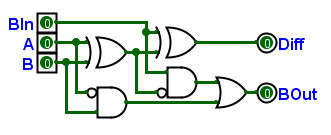
\includegraphics[width=\maxwidth{.95\linewidth}]{gfx/08_09}
	\caption{Subtractor}
	\label{fig:08_09}
\end{figure}

\subsection{Cascading Subtractors}
\label{CL:subsec:cascading_subtractors}

The full subtractor developed above will only subtract two one-bit numbers along with an optional borrow bit; however, those subtractors can be cascaded such that a subtractor of any bit width can be easily created. Figure \ref{fig:08_10} shows a four-bit subtractor created by cascading four one-bit subtractors.

\begin{figure}[H]
	\centering
	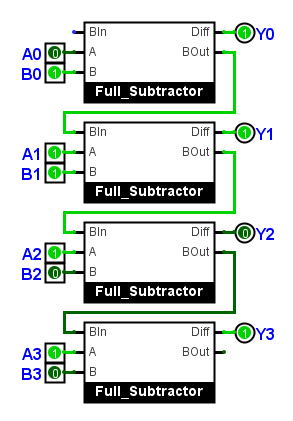
\includegraphics[width=\maxwidth{.95\linewidth}]{gfx/08_10}
	\caption{4-Bit Subtractor}
	\label{fig:08_10}
\end{figure}

This circuit would subtract a four bit number \emph{B} from \emph{A}. The subtractor is set up to solve $ 1110_2 - 0011_2 = 1011_2 $. Stage zero, at the top of the stack, subtracts bit zero of input \emph{B} from bit zero of input \emph{A} and then outputs bit zero of the difference, \emph{Y0}, along with a borrow-out bit. The borrow-out bit from stage zero is wired directly into the stage one's borrow-in port. That stage then subtracts bit one of input \emph{B} from bit one of input \emph{A} along with the borrow-in bit to create bit one of the sum, \emph{Y1}, along with a borrow-out bit. This process continues until all for bits have been subtracted. In the end, outputs \emph{Y0} - \emph{Y3} are combined to create a four-bit difference. The borrow-out bit of the last stage is not connected to anything but it could be used as the borrow-in bit for another device.

\subsection{Adder-Subtractor Circuit}
\label{CL:subsec:adder_subtractor_circuit}

It is remarkably easy to create a device that both adds and subtracts based on a single-bit control signal. Figure \ref{fig:08_11} is a 4-bit adder that was modified to become both an adder and subtractor. The circuit has been set up with this problem: $ 0101_2 - 0011_2 = 0010_2 $. 

\begin{figure}[H]
	\centering
	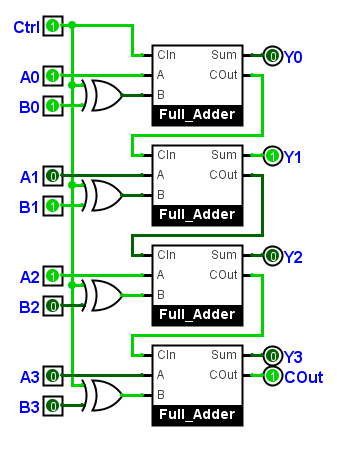
\includegraphics[width=\maxwidth{.95\linewidth}]{gfx/08_11}
	\caption{4-Bit Adder-Subtractor}
	\label{fig:08_11}
\end{figure}

To change an adder to an adder-subtractor makes use of the binary mathematics concept of subtracting by adding the twos complement (see Section \ref{MO:subsub:binary_subtraction_with_radix_complement} on page \pageref{MO:subsub:binary_subtraction_with_radix_complement}). The ``trick'' is to use the \textsf{XOR} gates on input \emph{B} to convert that input to its complement then the adder will subtract \emph{B} from \emph{A} instead of add. 

To create the twos complement of a binary number each of the bits are complemented and then one is added to the result (again, this process is described in Section \ref{MO:subsub:binary_subtraction_with_radix_complement}). Each of the \emph{B} input bits are wired through one input of an \textsf{XOR} gate. The other input of that gate is a \emph{Ctrl} (``Control'') bit. When \emph{Ctrl} is low then each of the \emph{B} inputs are transmitted through an \textsf{XOR} gate without change and the adder works as an adder. When \emph{Ctrl} is high then each of the \emph{B} inputs are complemented by an \textsf{XOR} gate such that the ones complement is created. However, \emph{Ctrl} is also wired to the \emph{CIn} input of the first stage which has the effect of adding one to the result and turn input \emph{B} into a twos complement number. Now the adder will subtract input \emph{B} from input \emph{A}.

In the end, the designer only needs to set \emph{Ctrl} to zero to make the circuit add or one to make the circuit subtract.

\subsection{Integrated Circuits}
\label{CL:subsec:adder_integrated_circuits}

In practice, circuit designers rarely build adders or subtractors. There are many different types of manufactured low-cost adders, subtractors, and adder/subtractor combinations available and designers usually find it easiest to use one of those circuits rather than re-invent the proverbial wheel. A quick look at Wikipedia\footnote{\url{https://www.wikipedia.com/en/List_of_7400_series_integrated_circuits}} found this list of adders:

\begin{itemize}
	\item $ 7480 $, gated full adder
	\item $ 7482 $, two-bit binary full adder
	\item $ 7483 $, four-bit binary full adder
	\item $ 74183 $, dual carry-save full adder
	\item $ 74283 $, four-bit binary full adder
	\item $ 74385 $, quad four-bit adder/subtractor
	\item $ 74456 $, BCD adder
\end{itemize}

In addition to adder circuits, designers can also opt to use an \gls{alu} \gls{ic}.

\section{Arithmetic Logic Units}
\label{CL:sec:arithmetic_and_logic_units}

An \gls{alu} is a specialized \gls{ic} that performs all arithmetic and logic functions needed in a device. Most \glspl{alu} will carry out dozens of different functions like the following few examples from a $ 74181 $ \gls{alu} (assume that the ALU has two inputs, $ A $ and $ B $, and one output, $ F $):

\begin{itemize}
  \item \lstinline[columns=fixed]|F = NOT A|
  \item \lstinline[columns=fixed]|F = A NAND B|
  \item \lstinline[columns=fixed]|F = (NOT A) OR B|
  \item \lstinline[columns=fixed]|F = B|
  \item \lstinline[columns=fixed]|F = (NOT A) AND B|
  \item \lstinline[columns=fixed]|F = A - 1|
  \item \lstinline[columns=fixed]|F = A - B|
  \item \lstinline[columns=fixed]|F = AB - 1|
  \item \lstinline[columns=fixed]|F = -1|
\end{itemize}

\glspl{alu} are very important in many devices, in fact, they are at the core of a \gls{cpu}. Because they are readily available at low cost, most designers will use a commercially-produced \gls{alu} in a project rather than try to create their own.

A quick look at Wikipedia\footnote{\url{https://www.wikipedia.com/en/List_of_7400_series_integrated_circuits}} found this list of \glspl{alu}:

\begin{itemize}
  \item $ 74181 $, four-bit arithmetic logic unit and function generator
  \item $ 74381 $, four-bit arithmetic logic unit/function generator with generate and propagate outputs
  \item $ 74382 $, four-bit arithmetic logic unit/function generator with ripple carry and overflow outputs
  \item $ 74881 $, Arithmetic logic unit
\end{itemize}

\section{Comparators}
\label{CL:sec:comparators}

A comparator compares two binary numbers, \emph{A} and \emph{B}. One of three outputs is generated by the comparison: \lstinline[]|A = B, A > B, A < B|. A one-bit comparator uses a combination of \textsf{AND} gates, \textsf{NOT} gates, and an \textsf{XNOR} gate to generate a \emph{True} output for each of the three comparisons: 

\begin{table}[H]
	\sffamily
	\newcommand{\head}[1]{\textcolor{white}{\textbf{#1}}}    
	\begin{center}
		\rowcolors{1}{gray!10}{white} % Color every other line a light gray
		\begin{tabular}{cc} 
			$ A=B $ & $ (A \odot B)' $ \\
			$ A > B $ & $ AB' $ \\
			$ A < B $ & $ A'B $
		\end{tabular}
	\end{center}
	\caption{One-Bit Comparator Functions}
	\label{CL:tab:one-bit_comparator_functions}
\end{table}

Figure \ref{fig:08_12} is the logic diagram for a one-bit comparator.  

\begin{figure}[H]
	\centering
	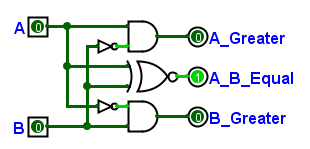
\includegraphics[width=\maxwidth{.95\linewidth}]{gfx/08_12}
	\caption{One-Bit Comparator}
	\label{fig:08_12}
\end{figure}

To compare numbers larger than one bit requires a more involved analysis of the problem. First, a truth table is developed for every possible combination of two 2-bit numbers, \emph{A} and \emph{B}.

\begin{table}[H]
	\sffamily
	\newcommand{\head}[1]{\textcolor{white}{\textbf{#1}}}		
	\begin{center}
		\rowcolors{2}{gray!10}{white} % Color every other line a light gray
		\begin{tabular}{cccc|ccc} 
			\rowcolor{black!75}
			\multicolumn{4}{c}{\head{Inputs}} & \multicolumn{3}{c}{\head{Outputs}} \\
			$A1$ & $A0$ & $B1$ & $B0$ & $A<B$ & $A=B$ & $A>B$ \\
			\hline
			0 & 0 & 0 & 0 & 0 & 1 & 0 \\
			0 & 0 & 0 & 1 & 1 & 0 & 0 \\
			0 & 0 & 1 & 0 & 1 & 0 & 0 \\
			0 & 0 & 1 & 1 & 1 & 0 & 0 \\
			0 & 1 & 0 & 0 & 0 & 0 & 1 \\
			0 & 1 & 0 & 1 & 0 & 1 & 0 \\
			0 & 1 & 1 & 0 & 1 & 0 & 0 \\
			0 & 1 & 1 & 1 & 1 & 0 & 0 \\
			1 & 0 & 0 & 0 & 0 & 0 & 1 \\
			1 & 0 & 0 & 1 & 0 & 0 & 1 \\
			1 & 0 & 1 & 0 & 0 & 1 & 0 \\
			1 & 0 & 1 & 1 & 1 & 0 & 0 \\
			1 & 1 & 0 & 0 & 0 & 0 & 1 \\
			1 & 1 & 0 & 1 & 0 & 0 & 1 \\
			1 & 1 & 1 & 0 & 0 & 0 & 1 \\
			1 & 1 & 1 & 1 & 0 & 1 & 0 
		\end{tabular}
	\end{center}
	\caption{Truth Table for Two-Bit Comparator}
	\label{08:tab:two_bit_comparator}
\end{table}

Next, Karnaugh Maps are developed for each of the three outputs.

%%%%%%%%%%%%%%%%%%%%%%%%%%%%%%%%%%%%%%%%%%%%%%%%%%%%%%%%%%%%%%
% K-Map #1 A>B
%%%%%%%%%%%%%%%%%%%%%%%%%%%%%%%%%%%%%%%%%%%%%%%%%%%%%%%%%%%%%%

\begin{figure}[H]
	\myfloatalign
	\begin{tikzpicture} [circuit logic US, scale=1.00]
	% make all path lines (the node shapes) a little thicker
	\tikzstyle{every path}=[line width=0.50mm]
	
	%********************************************************************
	% Adjust the settings below to display the 1's and rectangles
	%********************************************************************
	% Uncomment the appropriate lines below to insert ones where needed
	% Data Row 1
	% \node[] at (2.25,5.25) {\Huge $ 1 $}; % 00
	% \node[] at (3.75,5.25) {\Huge $ 1 $}; % 04
	% \node[] at (5.25,5.25) {\Huge $ 1 $}; % 12
	% \node[] at (6.75,5.25) {\Huge $ 1 $}; % 08
	% Data Row 2
	\node[] at (2.25,3.75) {\Huge $ 1 $}; % 01
	% \node[] at (3.75,3.75) {\Huge $ 1 $}; % 05
	% \node[] at (5.25,3.75) {\Huge $ 1 $}; % 13
	% \node[] at (6.75,3.75) {\Huge $ 1 $}; % 09
	% Data Row 3
	\node[] at (2.25,2.25) {\Huge $ 1 $}; % 03
	\node[] at (3.75,2.25) {\Huge $ 1 $}; % 07
	% \node[] at (5.25,2.25) {\Huge $ 1 $}; % 15
	\node[] at (6.75,2.25) {\Huge $ 1 $}; % 11
	% Data Row 4
	\node[] at (2.25,0.75) {\Huge $ 1 $}; % 02
	\node[] at (3.75,0.75) {\Huge $ 1 $}; % 06
	% \node[] at (5.25,0.75) {\Huge $ 1 $}; % 14
	% \node[] at (6.75,0.75) {\Huge $ 1 $}; % 10
	
	% The coords for each cell - this is used to start the rectangle box
	\coordinate (cell00) at (1.50,4.50); \coordinate (cell01) at (1.50,3.00);
	\coordinate (cell02) at (1.50,0.00); \coordinate (cell03) at (1.50,1.50);
	\coordinate (cell04) at (3.00,4.50); \coordinate (cell05) at (3.00,3.00);
	\coordinate (cell06) at (3.00,0.00); \coordinate (cell07) at (3.00,1.50);
	\coordinate (cell08) at (6.00,4.50); \coordinate (cell09) at (6.00,3.00);
	\coordinate (cell10) at (6.00,0.00); \coordinate (cell11) at (6.00,1.50);
	\coordinate (cell12) at (4.50,4.50); \coordinate (cell13) at (4.50,3.00);
	\coordinate (cell14) at (4.50,0.00); \coordinate (cell15) at (4.50,1.50);
	
	% Set the ``at'' to the lower-left cell of the rectangle using the coords defined above
	% Set the minimum height/width to (number of cells) * 1.5. May have to decrease 
	% these by 0.1 to cut the rectangle just inside the cell.
	\node [draw,
	color=red!70!black,
	fill=red!20!white,
	fill opacity=0.3,
	minimum height=2.9cm,
	minimum width=3.0cm,
	double,
	rounded corners,
	anchor=south west] at (cell02) {};
	
	\node [draw,
	color=blue!70!black,
	fill=blue!20!white,
	fill opacity=0.3,
	minimum height=2.9cm,
	minimum width=1.5cm,
	double,
	rounded corners,
	anchor=south west] at (cell03) {};
	
	\node [draw,
	color=green!70!black,
	fill=green!20!white,
	fill opacity=0.3,
	minimum height=1.4cm,
	minimum width=1.5cm,
	double,
	rounded corners,
	anchor=south west] at (cell11) {};
	
	\node [draw,
	color=green!70!black,
	fill=green!20!white,
	fill opacity=0.3,
	minimum height=1.4cm,
	minimum width=1.5cm,
	double,
	rounded corners,
	anchor=south west] at (cell03) {};
	
	%********************************************************************
	% Shouldn't need to adjust anything below this point - this is just
	% the grid and the minterms.
	%********************************************************************	
	% Text in top-Left cell
	\node[] at (0.55,6.35) { $ \mathsf{ \mathbf{A1A0} } $ }; % CD
	\node[] at (1.05,7.05) { $ \mathsf{ \mathbf{B1B0} } $ }; % AB
	
	% Populate the top row header
	% In the following, the foreach lists a location/text pair
	% The the draw line draws the text at each location
	\foreach \loc/\txt in {(2.25,6.75)/{00},(3.75,6.75)/{01},(5.25,6.75)/{11},(6.75,6.75)/{10}}
	\draw \loc node{\Huge $\txt$};
	
	% Populate the header in column one
	\foreach \loc/\txt in {(0.75,5.25)/{00},(0.75,3.75)/{01},(0.75,2.25)/{11},(0.75,0.75)/{10}}
	\draw \loc node{\Huge $\txt$};
	
	% Populate the minterms
	\foreach \loc/\txt in { (2.75,4.75)/{00} , (4.25,4.75)/{04} , (5.75,4.75)/{12} , (7.25,4.75)/{08} ,
		(2.75,3.25)/{01} , (4.25,3.25)/{05} , (5.75,3.25)/{13} , (7.25,3.25)/{09} ,
		(2.75,1.75)/{03} , (4.25,1.75)/{07} , (5.75,1.75)/{15} , (7.25,1.75)/{11} ,
		(2.75,0.25)/{02} , (4.25,0.25)/{06} , (5.75,0.25)/{14} , (7.25,0.25)/{10} }
	\draw \loc node{ \color{blue!90!black} \small{ $\txt$ }};
	
	% Draw the lines
	\draw
	% Finish drawing the grid
	[step=1.5cm,black,thin] (0,0) grid (7.5,7.5) % The Grid
	(0.0,7.5) -- (1.5,6.0) % Diagonal in the top left cell
	(1.5,6.10) -- (7.50,6.10) % Double line under top header row
	(1.40,0.0) -- (1.40,6.0) % Double line on left of header column one
	;
	\end{tikzpicture}
	\caption{K-Map For $A>B$}
	\label{kmap:08_05}
\end{figure}

%%%%%%%%%%%%%%%%%%%%%%%%%%%%%%%%%%%%%%%%%%%%%%%%%%%%%%%%%%%%%%
% K-Map #2 A=B
%%%%%%%%%%%%%%%%%%%%%%%%%%%%%%%%%%%%%%%%%%%%%%%%%%%%%%%%%%%%%%

\begin{figure}[H]
	\myfloatalign
	\begin{tikzpicture} [circuit logic US, scale=1.00]
	% make all path lines (the node shapes) a little thicker
	\tikzstyle{every path}=[line width=0.50mm]
	
	%********************************************************************
	% Adjust the settings below to display the 1's and rectangles
	%********************************************************************
	% Uncomment the appropriate lines below to insert ones where needed
	% Data Row 1
	\node[] at (2.25,5.25) {\Huge $ 1 $}; % 00
	% \node[] at (3.75,5.25) {\Huge $ 1 $}; % 04
	% \node[] at (5.25,5.25) {\Huge $ 1 $}; % 12
	% \node[] at (6.75,5.25) {\Huge $ 1 $}; % 08
	% Data Row 2
	% \node[] at (2.25,3.75) {\Huge $ 1 $}; % 01
	\node[] at (3.75,3.75) {\Huge $ 1 $}; % 05
	% \node[] at (5.25,3.75) {\Huge $ 1 $}; % 13
	% \node[] at (6.75,3.75) {\Huge $ 1 $}; % 09
	% Data Row 3
	% \node[] at (2.25,2.25) {\Huge $ 1 $}; % 03
	% \node[] at (3.75,2.25) {\Huge $ 1 $}; % 07
	\node[] at (5.25,2.25) {\Huge $ 1 $}; % 15
	% \node[] at (6.75,2.25) {\Huge $ 1 $}; % 11
	% Data Row 4
	% \node[] at (2.25,0.75) {\Huge $ 1 $}; % 02
	% \node[] at (3.75,0.75) {\Huge $ 1 $}; % 06
	% \node[] at (5.25,0.75) {\Huge $ 1 $}; % 14
	\node[] at (6.75,0.75) {\Huge $ 1 $}; % 10
	
	% The coords for each cell - this is used to start the rectangle box
	\coordinate (cell00) at (1.50,4.50); \coordinate (cell01) at (1.50,3.00);
	\coordinate (cell02) at (1.50,0.00); \coordinate (cell03) at (1.50,1.50);
	\coordinate (cell04) at (3.00,4.50); \coordinate (cell05) at (3.00,3.00);
	\coordinate (cell06) at (3.00,0.00); \coordinate (cell07) at (3.00,1.50);
	\coordinate (cell08) at (6.00,4.50); \coordinate (cell09) at (6.00,3.00);
	\coordinate (cell10) at (6.00,0.00); \coordinate (cell11) at (6.00,1.50);
	\coordinate (cell12) at (4.50,4.50); \coordinate (cell13) at (4.50,3.00);
	\coordinate (cell14) at (4.50,0.00); \coordinate (cell15) at (4.50,1.50);
	
	% Set the ``at'' to the lower-left cell of the rectangle using the coords defined above
	% Set the minimum height/width to (number of cells) * 1.5. May have to decrease 
	% these by 0.1 to cut the rectangle just inside the cell.
	\node [draw,
	color=red!70!black,
	fill=red!20!white,
	fill opacity=0.3,
	minimum height=1.4cm,
	minimum width=1.5cm,
	double,
	rounded corners,
	anchor=south west] at (cell00) {};
	
	\node [draw,
	color=blue!70!black,
	fill=blue!20!white,
	fill opacity=0.3,
	minimum height=1.4cm,
	minimum width=1.5cm,
	double,
	rounded corners,
	anchor=south west] at (cell05) {};
	
	\node [draw,
	color=yellow!70!black,
	fill=yellow!20!white,
	fill opacity=0.3,
	minimum height=1.4cm,
	minimum width=1.5cm,
	double,
	rounded corners,
	anchor=south west] at (cell15) {};
	
	\node [draw,
	color=green!70!black,
	fill=green!20!white,
	fill opacity=0.3,
	minimum height=1.4cm,
	minimum width=1.5cm,
	double,
	rounded corners,
	anchor=south west] at (cell10) {};
	
	%********************************************************************
	% Shouldn't need to adjust anything below this point - this is just
	% the grid and the minterms.
	%********************************************************************	
	% Text in top-Left cell
	\node[] at (0.55,6.35) { $ \mathsf{ \mathbf{A1A0} } $ }; % CD
	\node[] at (1.05,7.05) { $ \mathsf{ \mathbf{B1B0} } $ }; % AB
	
	% Populate the top row header
	% In the following, the foreach lists a location/text pair
	% The the draw line draws the text at each location
	\foreach \loc/\txt in {(2.25,6.75)/{00},(3.75,6.75)/{01},(5.25,6.75)/{11},(6.75,6.75)/{10}}
	\draw \loc node{\Huge $\txt$};
	
	% Populate the header in column one
	\foreach \loc/\txt in {(0.75,5.25)/{00},(0.75,3.75)/{01},(0.75,2.25)/{11},(0.75,0.75)/{10}}
	\draw \loc node{\Huge $\txt$};
	
	% Populate the minterms
	\foreach \loc/\txt in { (2.75,4.75)/{00} , (4.25,4.75)/{04} , (5.75,4.75)/{12} , (7.25,4.75)/{08} ,
		(2.75,3.25)/{01} , (4.25,3.25)/{05} , (5.75,3.25)/{13} , (7.25,3.25)/{09} ,
		(2.75,1.75)/{03} , (4.25,1.75)/{07} , (5.75,1.75)/{15} , (7.25,1.75)/{11} ,
		(2.75,0.25)/{02} , (4.25,0.25)/{06} , (5.75,0.25)/{14} , (7.25,0.25)/{10} }
	\draw \loc node{ \color{blue!90!black} \small{ $\txt$ }};
	
	% Draw the lines
	\draw
	% Finish drawing the grid
	[step=1.5cm,black,thin] (0,0) grid (7.5,7.5) % The Grid
	(0.0,7.5) -- (1.5,6.0) % Diagonal in the top left cell
	(1.5,6.10) -- (7.50,6.10) % Double line under top header row
	(1.40,0.0) -- (1.40,6.0) % Double line on left of header column one
	;
	\end{tikzpicture}
	\caption{K-Map For $A=B$}
	\label{kmap:08_06}
\end{figure}

%%%%%%%%%%%%%%%%%%%%%%%%%%%%%%%%%%%%%%%%%%%%%%%%%%%%%%%%%%%%%%
% K-Map #3 A<B
%%%%%%%%%%%%%%%%%%%%%%%%%%%%%%%%%%%%%%%%%%%%%%%%%%%%%%%%%%%%%%

\begin{figure}[H]
	\myfloatalign
	\begin{tikzpicture} [circuit logic US, scale=1.00]
	% make all path lines (the node shapes) a little thicker
	\tikzstyle{every path}=[line width=0.50mm]
	
	%********************************************************************
	% Adjust the settings below to display the 1's and rectangles
	%********************************************************************
	% Uncomment the appropriate lines below to insert ones where needed
	% Data Row 1
	% \node[] at (2.25,5.25) {\Huge $ 1 $}; % 00
	\node[] at (3.75,5.25) {\Huge $ 1 $}; % 04
	\node[] at (5.25,5.25) {\Huge $ 1 $}; % 12
	\node[] at (6.75,5.25) {\Huge $ 1 $}; % 08
	% Data Row 2
	% \node[] at (2.25,3.75) {\Huge $ 1 $}; % 01
	% \node[] at (3.75,3.75) {\Huge $ 1 $}; % 05
	\node[] at (5.25,3.75) {\Huge $ 1 $}; % 13
	\node[] at (6.75,3.75) {\Huge $ 1 $}; % 09
	% Data Row 3
	% \node[] at (2.25,2.25) {\Huge $ 1 $}; % 03
	% \node[] at (3.75,2.25) {\Huge $ 1 $}; % 07
	% \node[] at (5.25,2.25) {\Huge $ 1 $}; % 15
	% \node[] at (6.75,2.25) {\Huge $ 1 $}; % 11
	% Data Row 4
	% \node[] at (2.25,0.75) {\Huge $ 1 $}; % 02
	% \node[] at (3.75,0.75) {\Huge $ 1 $}; % 06
	\node[] at (5.25,0.75) {\Huge $ 1 $}; % 14
	% \node[] at (6.75,0.75) {\Huge $ 1 $}; % 10
	
	% The coords for each cell - this is used to start the rectangle box
	\coordinate (cell00) at (1.50,4.50); \coordinate (cell01) at (1.50,3.00);
	\coordinate (cell02) at (1.50,0.00); \coordinate (cell03) at (1.50,1.50);
	\coordinate (cell04) at (3.00,4.50); \coordinate (cell05) at (3.00,3.00);
	\coordinate (cell06) at (3.00,0.00); \coordinate (cell07) at (3.00,1.50);
	\coordinate (cell08) at (6.00,4.50); \coordinate (cell09) at (6.00,3.00);
	\coordinate (cell10) at (6.00,0.00); \coordinate (cell11) at (6.00,1.50);
	\coordinate (cell12) at (4.50,4.50); \coordinate (cell13) at (4.50,3.00);
	\coordinate (cell14) at (4.50,0.00); \coordinate (cell15) at (4.50,1.50);
	
	% Set the ``at'' to the lower-left cell of the rectangle using the coords defined above
	% Set the minimum height/width to (number of cells) * 1.5. May have to decrease 
	% these by 0.1 to cut the rectangle just inside the cell.
	\node [draw,
	color=red!70!black,
	fill=red!20!white,
	fill opacity=0.3,
	minimum height=2.9cm,
	minimum width=3.0cm,
	double,
	rounded corners,
	anchor=south west] at (cell13) {};
	
	\node [draw,
	color=blue!70!black,
	fill=blue!20!white,
	fill opacity=0.3,
	minimum height=1.4cm,
	minimum width=3.0cm,
	double,
	rounded corners,
	anchor=south west] at (cell04) {};
	
	\node [draw,
	color=green!70!black,
	fill=green!20!white,
	fill opacity=0.3,
	minimum height=1.4cm,
	minimum width=1.5cm,
	double,
	rounded corners,
	anchor=south west] at (cell14) {};
	
	\node [draw,
	color=green!70!black,
	fill=green!20!white,
	fill opacity=0.3,
	minimum height=1.4cm,
	minimum width=1.5cm,
	double,
	rounded corners,
	anchor=south west] at (cell12) {};
	
	%********************************************************************
	% Shouldn't need to adjust anything below this point - this is just
	% the grid and the minterms.
	%********************************************************************	
	% Text in top-Left cell
	\node[] at (0.55,6.35) { $ \mathsf{ \mathbf{A1A0} } $ }; % CD
	\node[] at (1.05,7.05) { $ \mathsf{ \mathbf{B1B0} } $ }; % AB
	
	% Populate the top row header
	% In the following, the foreach lists a location/text pair
	% The the draw line draws the text at each location
	\foreach \loc/\txt in {(2.25,6.75)/{00},(3.75,6.75)/{01},(5.25,6.75)/{11},(6.75,6.75)/{10}}
	\draw \loc node{\Huge $\txt$};
	
	% Populate the header in column one
	\foreach \loc/\txt in {(0.75,5.25)/{00},(0.75,3.75)/{01},(0.75,2.25)/{11},(0.75,0.75)/{10}}
	\draw \loc node{\Huge $\txt$};
	
	% Populate the minterms
	\foreach \loc/\txt in { (2.75,4.75)/{00} , (4.25,4.75)/{04} , (5.75,4.75)/{12} , (7.25,4.75)/{08} ,
		(2.75,3.25)/{01} , (4.25,3.25)/{05} , (5.75,3.25)/{13} , (7.25,3.25)/{09} ,
		(2.75,1.75)/{03} , (4.25,1.75)/{07} , (5.75,1.75)/{15} , (7.25,1.75)/{11} ,
		(2.75,0.25)/{02} , (4.25,0.25)/{06} , (5.75,0.25)/{14} , (7.25,0.25)/{10} }
	\draw \loc node{ \color{blue!90!black} \small{ $\txt$ }};
	
	% Draw the lines
	\draw
	% Finish drawing the grid
	[step=1.5cm,black,thin] (0,0) grid (7.5,7.5) % The Grid
	(0.0,7.5) -- (1.5,6.0) % Diagonal in the top left cell
	(1.5,6.10) -- (7.50,6.10) % Double line under top header row
	(1.40,0.0) -- (1.40,6.0) % Double line on left of header column one
	;
	\end{tikzpicture}
	\caption{K-Map For $A=B$}
	\label{kmap:08_07}
\end{figure}

Given the above K-Maps, the following Boolean Equations can be derived.
\begin{align}
\label{08:eq:comparator}
A<B &: A1'B1 + A0'B1B0 + A1'A0'B0 \\
\nonumber
A=B &: (A0 \odot B0) (A1 \odot B1) \\
\nonumber
A>B &: A1B1' + A0B1'B0' + A1A0B0'
\end{align}

The above Boolean expressions can be used to create the circuit in Figure \ref{fig:08_13}.

\begin{figure}[H]
	\centering
	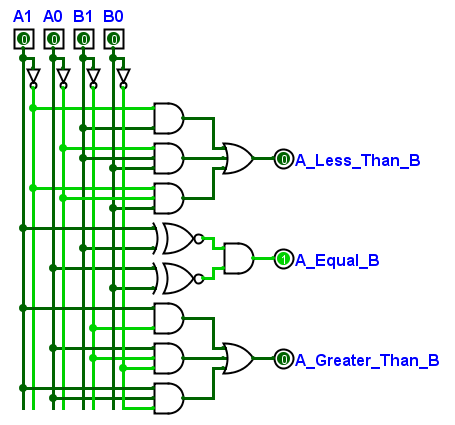
\includegraphics[width=\maxwidth{.95\linewidth}]{gfx/08_13}
	\caption{Two-Bit Comparator}
	\label{fig:08_13}
\end{figure}

